% !TEX root = ./pkMain.tex
\mode*


\frame{
\mode<presentation>{
\begin{tikzpicture}[remember picture, overlay]
\node[inner sep=0pt,xshift=0cm] at (current page.center){
\tikz \draw[step=2mm,black!50] (0,0) grid (126mm,94mm);
};
{
\node[coordinate] at (1cm,-3.55cm) (start) {};
\node[coordinate] at (1cm,3cm) (end) {};
\node[coordinate] at (10cm,-3.55cm) (endy) {};
\draw[->,thick] (start)--(end);
\draw[->,thick] (start)--(endy);
};
\end{tikzpicture}
}
\frametitle{Konzentration am Wirkort $\Rightarrow$ Wirkung}

\note<1>{
\begin{itemize}
\item
Rezeptoren - endliche Zahl
\item
H\"ohere Konzentration: Keine zus\"atzliche Wirkung
\item
Begriff der Potenz: $\neq$ St\"arke: Bedeutung - Zusammenhang zu Sensitivit\"at
\item
Therapeutische Fenster
\item
Vorstellung haben  wie die Kurve bei einem Patienten verl\"auft. Steilheit absch\"atzen.
\item
Verstehen warum aufwachen so unterschiedlich sein kann
\end{itemize}
}
\infina
}

\mode<article>{
\vspace{1cm}
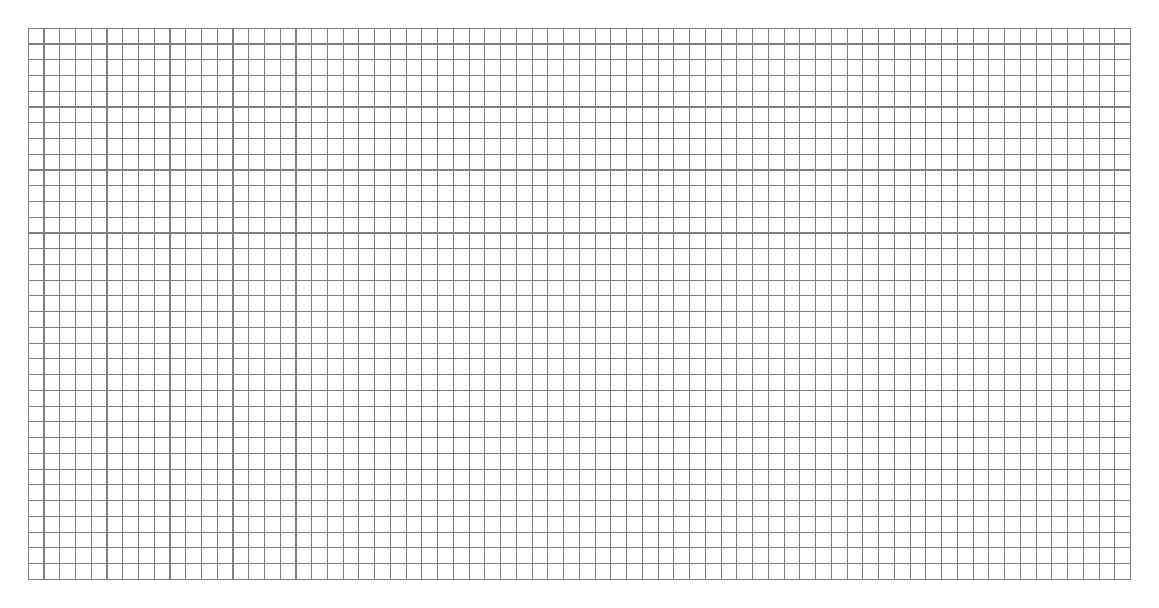
\begin{tikzpicture}[auto]
\node[inner sep=0pt,xshift=0cm] at (current page.center){
\tikz \draw[step=2mm,black!50] (0,0) grid (140mm,70mm);
};
\end{tikzpicture}
}

